\chapter{Theoretical introduction}\label{chap:Theory}
\minitoc
This thesis presents the measurement of a Standard Model (SM) process. Therefore the first section of this chapter gives a small overview of this model. The proton structure (Sec.~\ref{sec:ProtStr}) and physics of W and Z bosons in proton collisions (Sec.~\ref{sec:TheoWZ}) are also discussed. Additionally, the predictions for $W\to l\nu$ and $Z \to ll$ cross sections are presented in Sec.~\ref{sec:TheoWZ}.

Several references were used for a preparation of this chapter, including \cite{QPrim, Okun}.
\section{The Standard Model}

The Standard Model is the model, that explains the interactions between the elementary particles. It provides our current best understanding of the particle physics and unifies the quantum mechanics, special relativity and a field theory. It was postulated by Weinberg and Salam in mid-1970\cite{SM1, SM2, SM3} and is successfully tested for the last 40 years. Despite the fact, that there are some unexplained phenomena in SM, such as dark matter\cite{Planck2015}, the SM describes almost all laboratory data. The summary of all SM production cross section measurements at \atlas experiment is given in Fig.~\ref{fig:SMxsec}. The results agree with SM prediction over several orders of magnitude, and no significant deviation from SM has been found yet.

\begin{figure}[!tpb]
\center{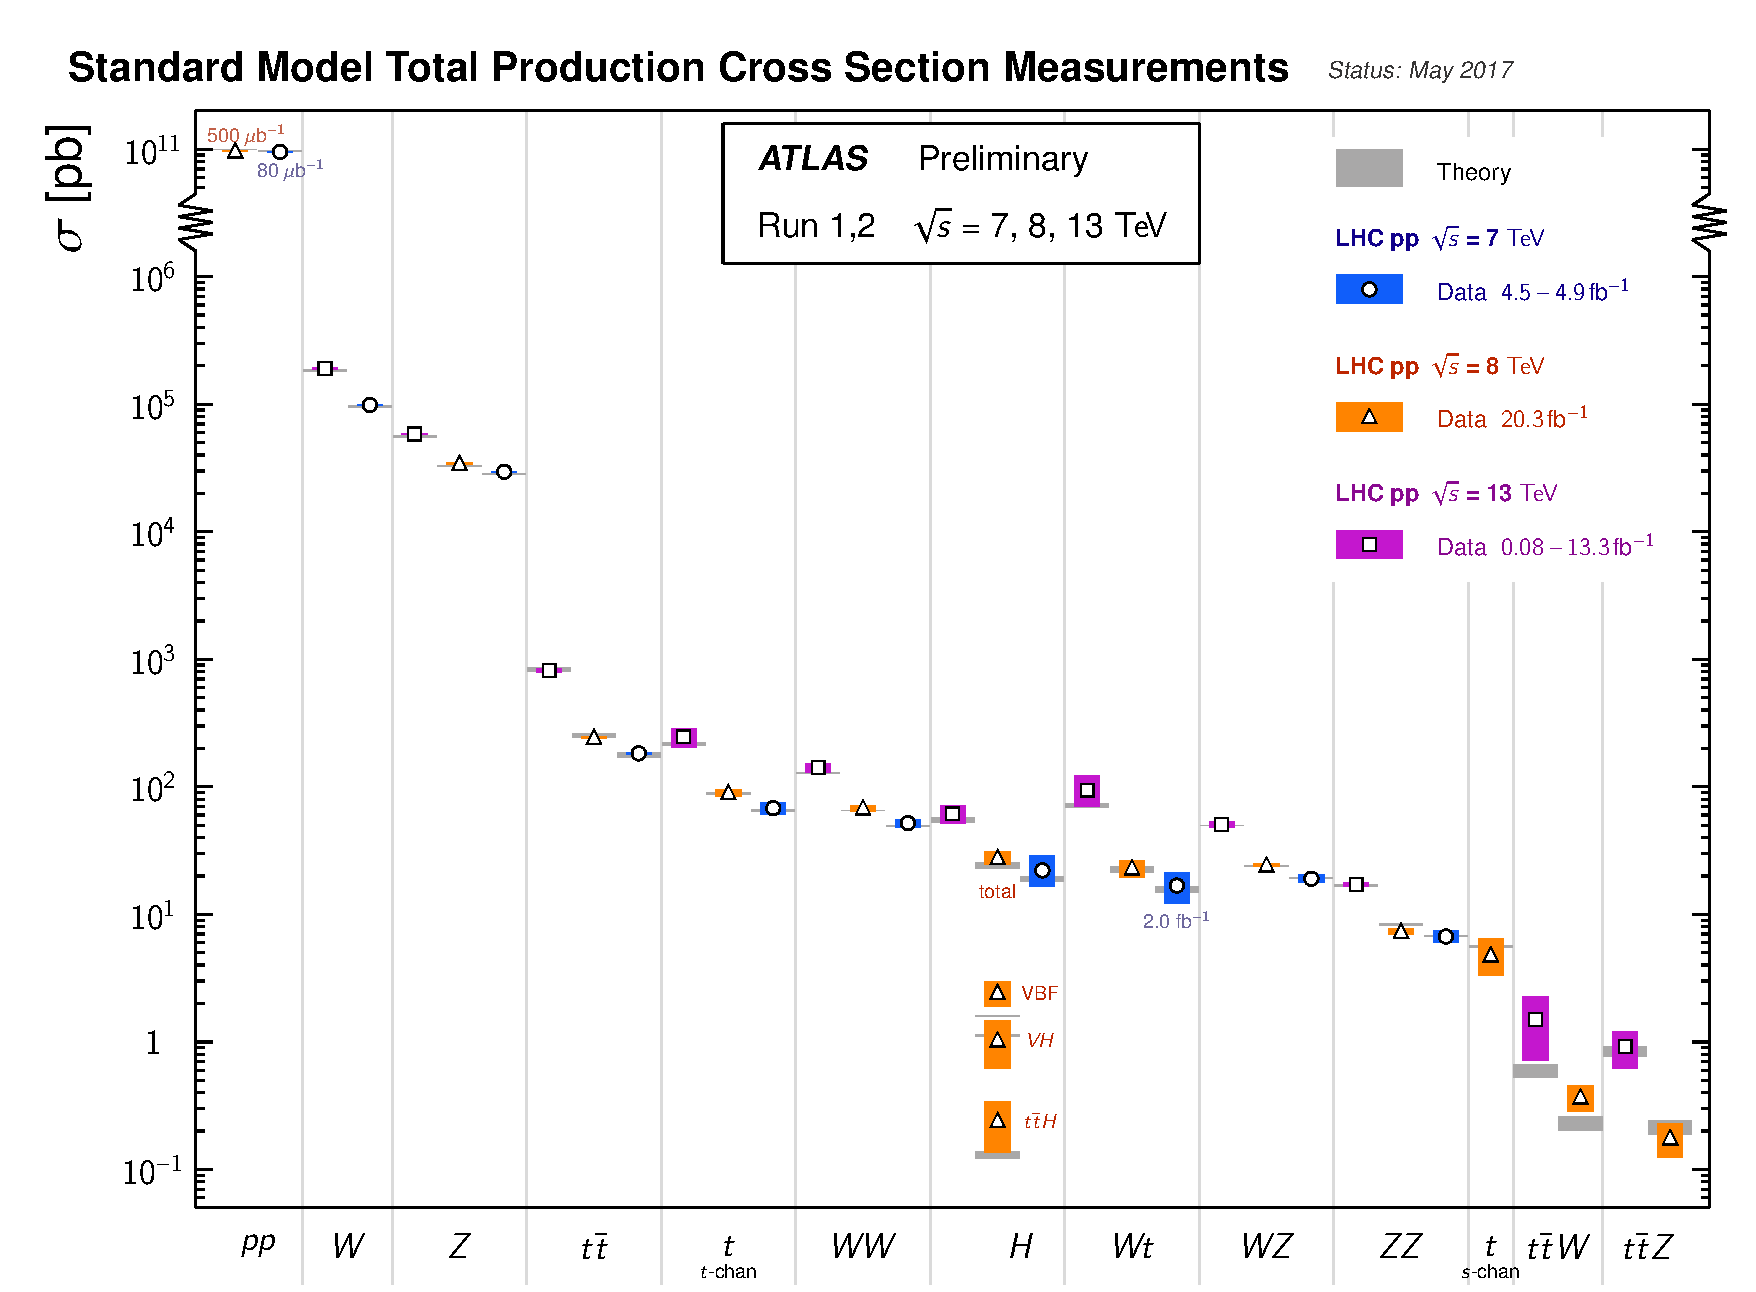
\includegraphics[width=0.9\linewidth]{Theory/SMXsec.pdf} }
\caption{Summary of SM production cross section measurements in the \atlas experiment, corrected for leptonic branching fractions, compared to the corresponding theoretical expectations. The amount of data used for each measurement is indicated close to the data point \cite{SMPubRes}.}
\label{fig:SMxsec}
\end{figure}

The SM postulates two types of fundamental particles: fermions and boson. Graphical representation of particles in SM with their masses and quantum numbers is shown in Fig.~\ref{fig:SMPart}. The fermions are the spin 1/2 particles that form the ordinary atomic matter. They can be further divided to leptons and quarks. Leptons can interact just electromagnetically and weakly, while quarks also undergo strong interactions. Both groups are divided into three separate generations.

\begin{figure}[!tbp]
\center{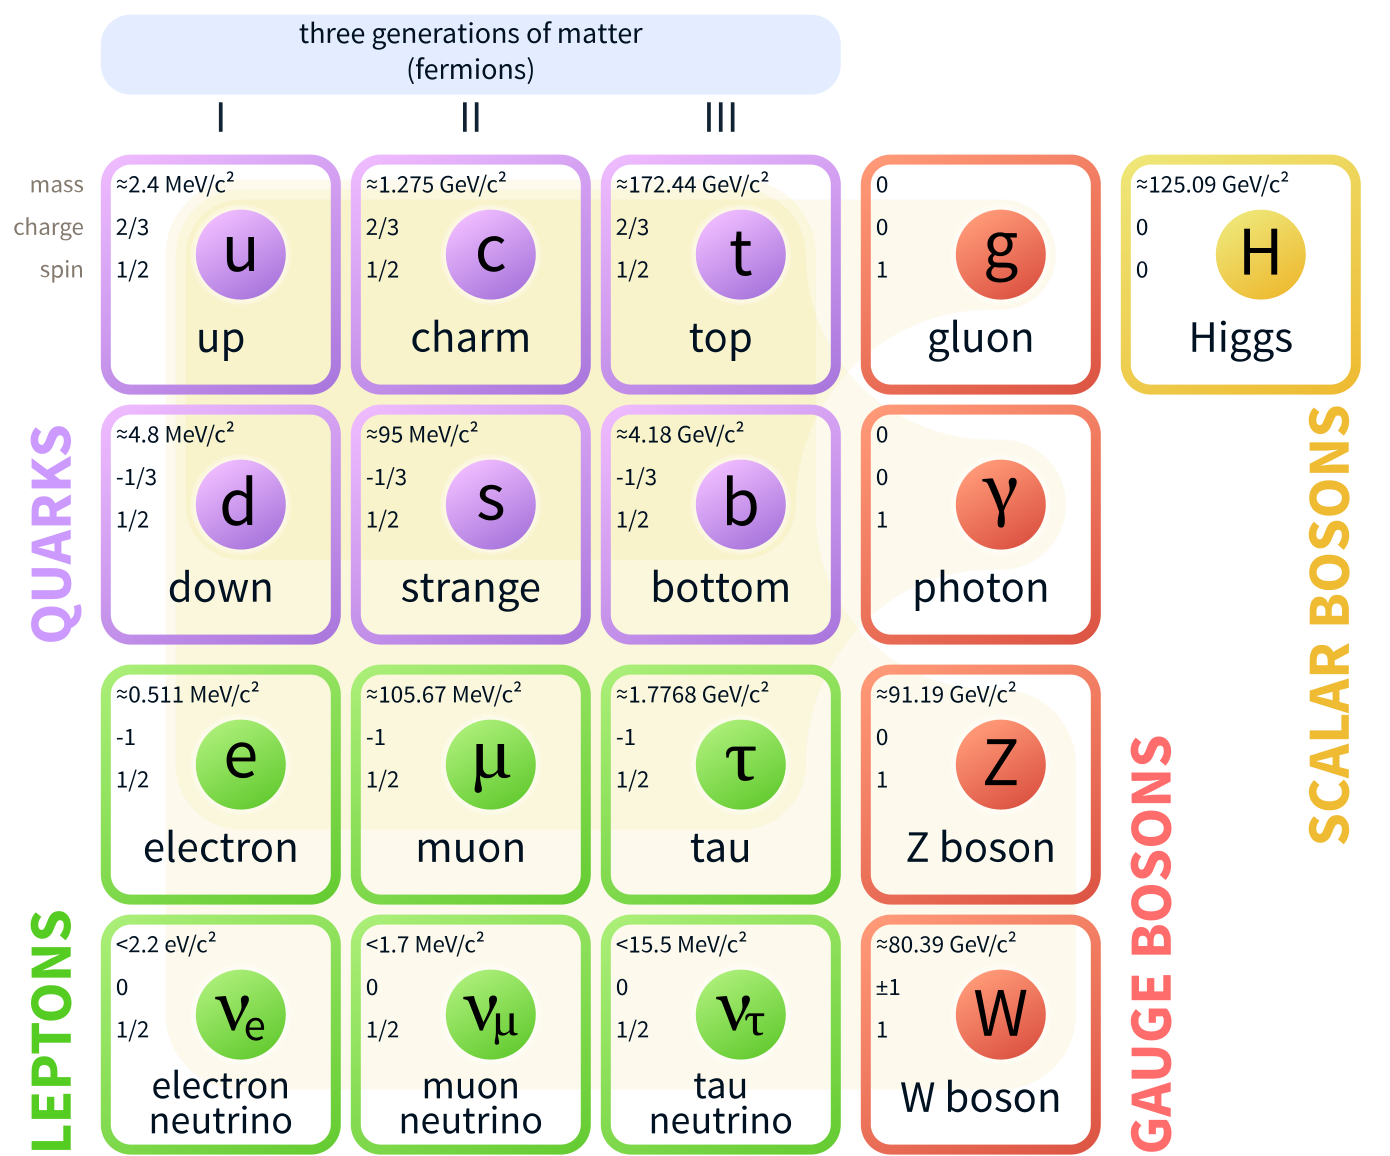
\includegraphics[width=0.5\linewidth]{Theory/SM.png} }
\caption{Fundamental particles of the Standard Model: three generations of fermions, the gauge bosons and Higgs boson \cite{SMParticles}.}
\label{fig:SMPart}
\end{figure}

The bosons are the carriers of the fundamental forces with the integer spin. Strong interactions are mediated by 8 massless gluons. The massless photons are carrying the electromagnetic interactions, while the W and Z-bosons are responsible for the weak forces. The last SM boson, observed in experimental data is the Higgs boson\cite{HiggsDiscoATLAS, HiggsDiscoCMS}. It is associated with Yukawa interactions, which are responsible for the fermion, W and Z-bosons masses. 

The SM is a \textit{non-abelian gauge theory}, meaning, that this theory is based on Lagrangian that is invariant under local and global transformations (called \textit{symmetries}). From the Noether theorem\cite{Noether1, Noether2} it is known, that each symmetry is connected to at least one conserved quantity. The symmetry group of SM is:
\begin{equation}
SU(3)_C \times SU(2)_L \times U(1)_Y,
\end{equation}
where hypercharge $Y$,  a left-handed helicity $L$ and  a color charge $C$ is the conserved quantum numbers of the corresponding symmetry group. The  $SU(2)_L \times U(1)_Y$ symmetry describes the electroweak (EW) theory, while the $SU(3)_C$ corresponds to the theory of strong interactions - Quantum Chromodynamics (QCD)\cite{QCD1, QCD2, QCD3}. 

The EW part of SM postulates three massless vector fields in $SU(2)_L$ - the isospin triplet of vector fields $W^1_\mu$, $W^2_\mu$, $W^3_\mu$ with the coupling constant $g$ and a single gauge field $B_\mu$ in $U(1)_L$ group with coupling strength $g'$. The $\gamma$ and the massive Z and W bosons are produced due to the spontaneous breaking of the electroweak gauge symmetry:
        \begin{align}
                \left(\gamma \atop Z^0 \right)
                &= \left(
            \begin{array}{cc}
            \cos \theta_W & \sin \theta_W \\
            -\sin \theta_W & \cos \theta_W
            \end{array}
            \right)
                \left(B \atop W^3 \right),
                 \\
                 W^\pm& = \frac{W^1 \pm i W^2}{\sqrt{2}},
        \end{align}
where  $\theta_W$ is the electroweak mixing angle which value is not predicted in the SM. The masses of Z and W bosons are connected by the relation:
\begin{equation}
M^2_W=cos^2_W M^2_Z.
\end{equation}


The QCD Lagrangian has only one free parameter - a \textit{strong coupling constant} $\alpha_s$. QCD theory uses a concept  similar to EW, however, it is more complicated because of the color charge of gluons, which allows them to interact with each other. The inclusion of the gluon--gluon interaction causes a  \textit{ultraviolet} (UV) divergences in the corresponding integrals. The renormalization procedure\cite{Renorm} allows to effectively remove them by introducing the arbitrary renormalization scale $\mu_R$. A typical scale for a physics process corresponds to the momentum transferred $Q^2$ between the interacting objects.

The QCD does not predict the value of $\alpha_s$, however it predicts its evolution with $\mu_{R}$ using the renormalization group equation (RGE):
\begin{equation}
\beta(\alpha_s) = \mu^2 \frac{d\alpha_s(\mu^2)}{d\mu^2}= - b_0 \alpha_s^2(\mu) - b_1 \alpha_s^3(\mu)-O(\alpha_s, n\geqslant4), 
\end{equation}
where the first coefficient is:
\begin{equation}
b_0 = \frac{33-2f}{12\pi},
\end{equation}
and $f=3$ is the number of quark flavors. This leads to the energy dependence of the strong coupling constant (showed in Fig.~\ref{fig:SMAlphaS}). The $\alpha_s$ value increases towards smaller scales, and it becomes small for higher $Q^2$. As a consequence, the quarks have a property of \textit{asymptotic freedom} and \textit{confinement}, meaning that they cannot be observed as free particles, but there are bound in QCD states, like a proton.

\begin{figure}[!tbp]
\center{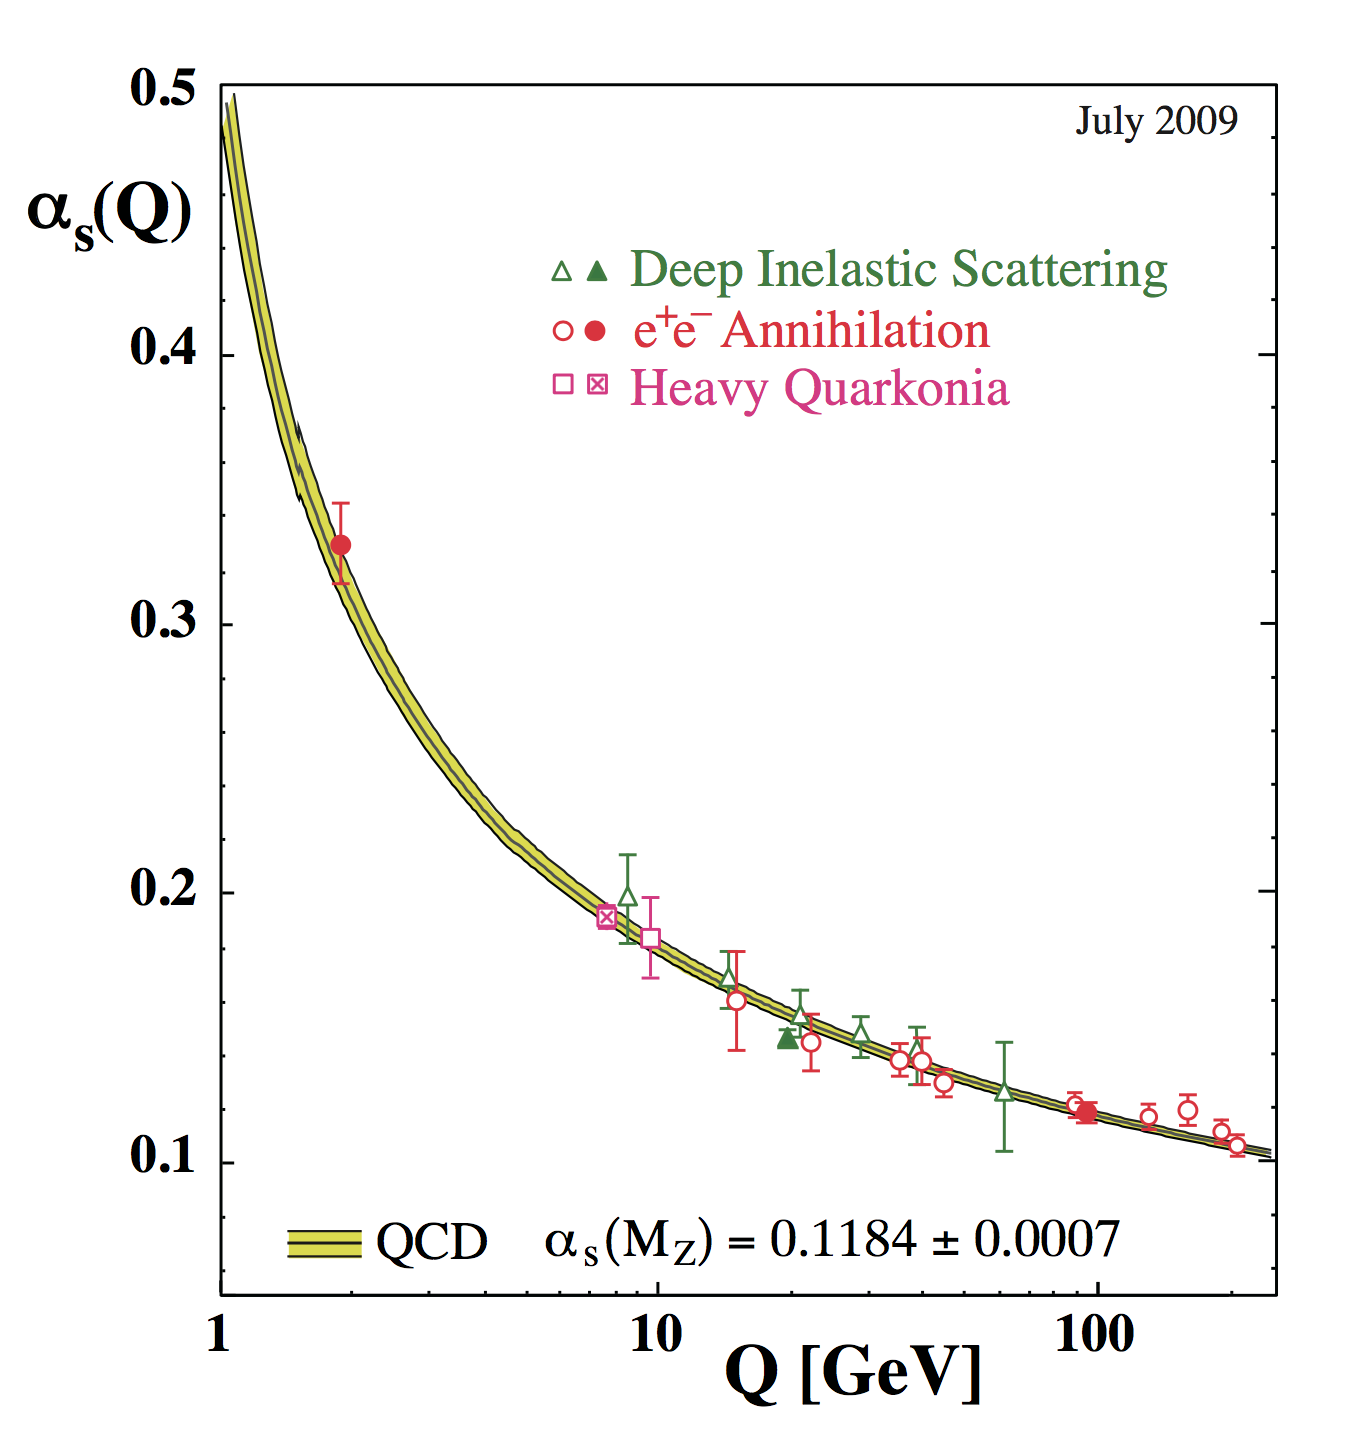
\includegraphics[width=0.5\linewidth]{Theory/alphaS.png} }
\caption{The coupling  of the strong interaction, $\alpha_s$, as a function of energy scale \cite{alphaS}.}
\label{fig:SMAlphaS}
\end{figure}


The physical quantities, like cross sections, do not depend on renormalization scale, however, the calculation on any perturbative order in $\alpha_s$ is a function of $\mu_R$. The cross section for the partonic interactions (or the \textit{partonic cross section}) $\sigma_{ab\to X}$ can be expressed perturbatively in $\alpha_s$ as:
\begin{equation}
\sigma_{ab\to X}=\hat{\sigma_0}+\alpha_{s}(\mu_R)\hat{\sigma_0}+\alpha^2_{s}(\mu_R)\hat{\sigma_2}+..., 
\end{equation}
where $\sigma_i$ is the $i$-th order contribution to the final cross section. The cross section, calculated at the lowest-order of the expansion is called the \textit{leading order} (LO) cross section. The calculation using the expansion of $\alpha_s$ up to the $i$-th order is called (next-to)$^i$ order (N$^i$LO) cross section. The inclusion of higher order corrections in the calculations allows to reduce the dependency on the renormalization scale. 


\section{Proton structure}\label{sec:ProtStr}
QCD predicts the cross section for the individual quark--quark interactions at different orders in $\alpha_s$. However, since quarks have not been observed in a free state, the tests of QCD  are possible using the experiments with hadrons (e.g. proton beams), so the internal quark composition in the hadron should be taken into account. 

In 1969 Feynman proposed a model of the proton structure called a parton model of the hadrons\cite{Feynman1969}. In this model he assumed that any hadron can be treated as a composition of point-like constituents called partons. In the high-energy scattering, the soft interaction between partons can be neglected, and therefore they can be treated as quasi-free in the collision. In this approximation, a total cross section for the process in hadron--hadron interaction can be written as a sum of all partonic cross sections:
\begin{equation}
\sigma = \sum_{i,j} \int dx_i dx_j f_i^{(P_1)}(x_i) f_j^{(P_2)}(x_j) \hat{\sigma}(x_ix_js), 
\end{equation}
where:
\begin{itemize}
\item $f_i^{(P_k)}(x_i)$ are the parton distribution functions (PDF) for both colliding hadrons. They describe the probability to find parton $i$  in hadron $k$ with a fraction of longitudinal momentum $x_i$;
\item $s=(P_1+P_2)^2$ is the center-of-mass energy of colliding hadrons;
\item $\hat{\sigma}(x_1x_2s)$ is the partonic cross section for a given scattering process, calculated in QCD.
\end{itemize}

The partons, which determine the quantum numbers of hadrons, are called \textit{valence quarks} ($u$ and $d$ quarks in case of the proton).  However, due to the quantum fluctuations, some number of quark pairs (of $u\bar{u}$, $d\bar{d}$, $c\bar{c}$ etc) with low momentum can be created. These quarks are called \textit{sea-quarks}. Due to the conservation of the total momentum and the quark flavor of a proton, the following sum rules are applicable for proton PDFs:
\begin{center}
$\int_0^1dx \sum_i x f_i^{(p)}(x) = 1$;\\
$\int_0^1dx (f_u^{(p)}(x)-f_{\bar{u}}^{(p)}(x)) = 1$;\\
$\int_0^1dx (f_d^{(p)}(x)-f_{\bar{d}}^{(p)}(x)) = 1$;\\
$\int_0^1dx (f_s^{(p)}(x)-f_{\bar{s}}^{(p)}(x)) = 1$,
\end{center}
where index $i$ runs over the quark flavors.

For the partonic cross sections, the soft emission of real and virtual gluons causes collinear singularities. However, it is possible to include initial state emissions below a given scale into non-perturbative parton distribution functions.  The cutoff parameter in this procedure is called a \textit{factorization scale} $\mu_F$ \cite{factscale}. This definition of PDFs is universal, i.e. they do not depend on a physics process. Similarly, the factorization scale $\mu_F$ is not a physical quantity, and the total partonic cross section should be independent of $\mu_f$. The typical choice of the scale is $\mu_R \approx \mu_R \approx Q^2$.

\begin{figure}[!tb]
\begin{minipage}[h]{0.4\linewidth}
\center{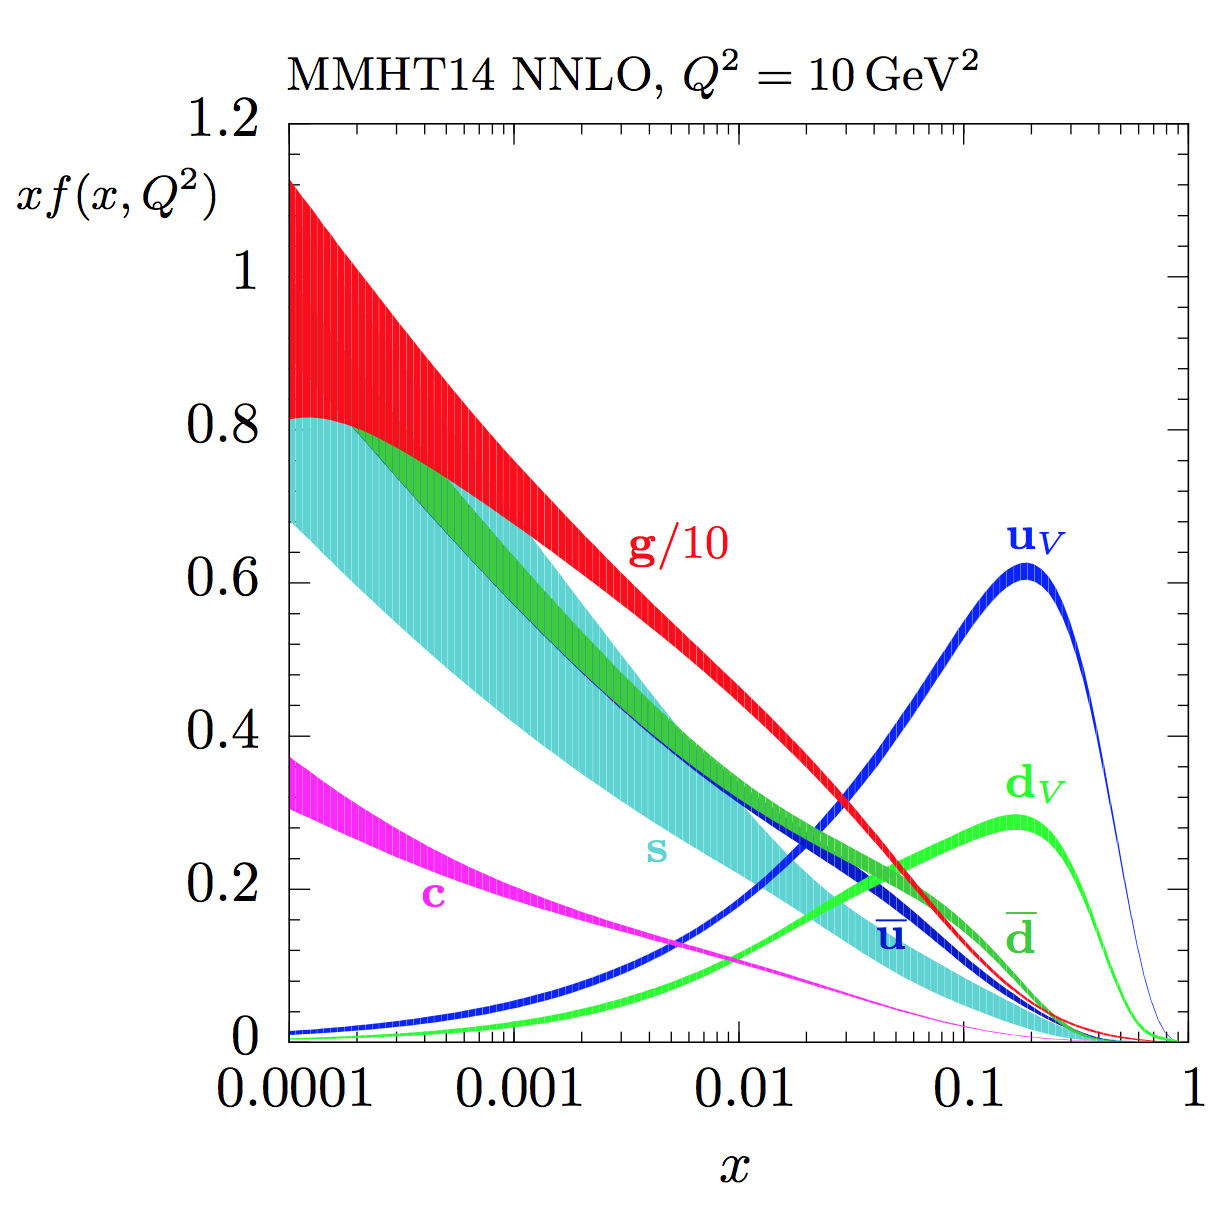
\includegraphics[width=1.0\linewidth]{Theory/MMHTPdfs.png} \\ a)}
\end{minipage}
\hfill
\begin{minipage}[h]{0.4\linewidth}
\center{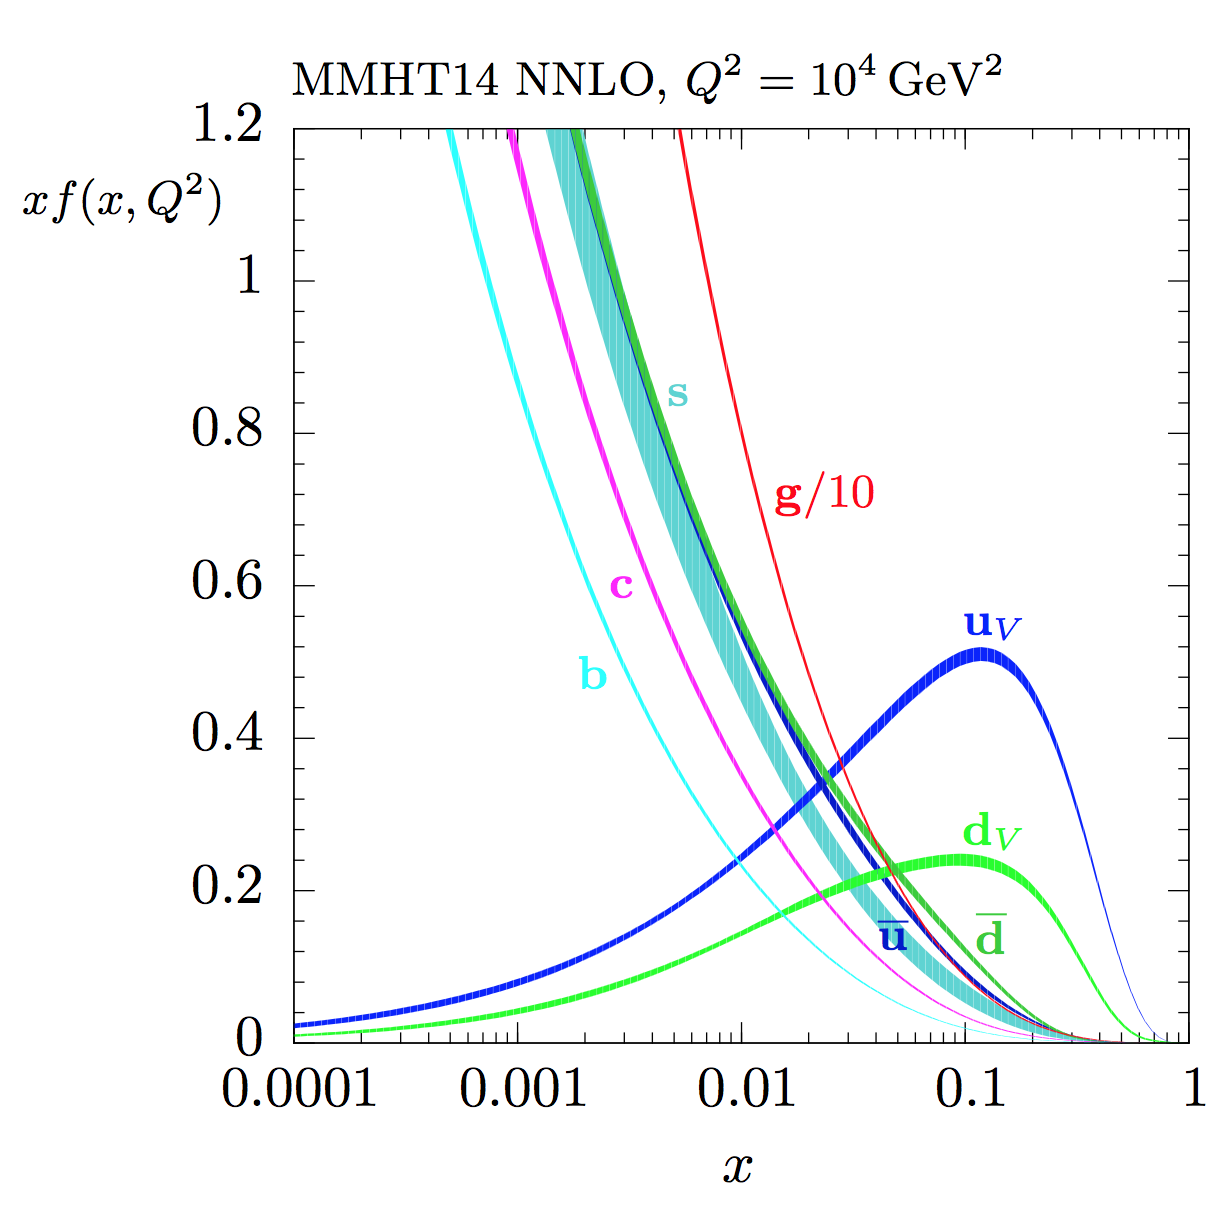
\includegraphics[width=1.0\linewidth]{Theory/MMHTPdfs2.png} \\ b)}
\end{minipage}
\caption{The MMHT2014 NNLO PDFs predictions at a) $Q^2 = 10 GeV^2$ and b) $Q^2 = 10^4 GeV^2$ with associated 68\% confidence-level uncertainty bands\cite{MMHT}.}
\label{fig:PFSMMHT}
\end{figure}

The parton density distributions cannot be calculated perturbatively in QCD and therefore need to be extracted from the experimental data. However, it is possible to predict the evolution of PDFs with factorization scale using the DLGAP evolution equations \cite{Gribov:1972ri}. An example of quark and gluon PDFs in the proton predicted by MMHT2015 NNLO\cite{MMHT} for different energy scales is shown in Fig.~\ref{fig:PFSMMHT}. The PDFs of valence ($u$ and $d$) quarks are reaching maximum at $x$=1/3, while the sea quark and gluon densities are rising at low-$x$. The contribution of the sea quarks and gluons becomes larger with increasing $Q^2$.



\section{Physics of W and Z bosons in pp collisions}\label{sec:TheoWZ}

The W and Z bosons are the massive vector bosons in the Standard Model.
They have been predicted by the Glasgow, Weinberg, Salam in 1960's\cite{SM1, SM2, SM3} and discovered in 1983 by UA1 and UA2 at CERN $p\bar{p}$ collider\cite{Wdisc1, Wdisc2, Wdisc3, Wdisc4}.  These particles are mediating weak interactions and decaying almost immediately ($t \approx 10^{-25}$ s). 

The leading order production mechanism of W/Z boson in pp collisions is a Drell-Yan mechanism, shown schematically in Fig.~\ref{fig:DY}. It is defined as an annihilation of the quark--antiquark pair through the exchange of a gauge boson, which decays into a fermion pair. A simplest example of this process is the production of the virtual photon $q\bar{q} \to \gamma^{*} \to l^+ l^-$. The corresponding cross section can be calculated using QED:
\begin{equation}
\hat{\sigma}(q\bar{q} \to \gamma^{*} \to e^+ e^-) = \frac{4\pi\alpha}{3\hat{s}}\frac{1}{N}Q^2_q,
\end{equation}
where $Q_q$ is the quark charge, $\hat{s}$ is the center-of-mass energy of the quark--antiquark system and $1/N=1/3$ is the color factor, coming from the fact, that quark and antiquark colors should match to create a color-singlet final state.

\begin{figure}[!tbp]
\center{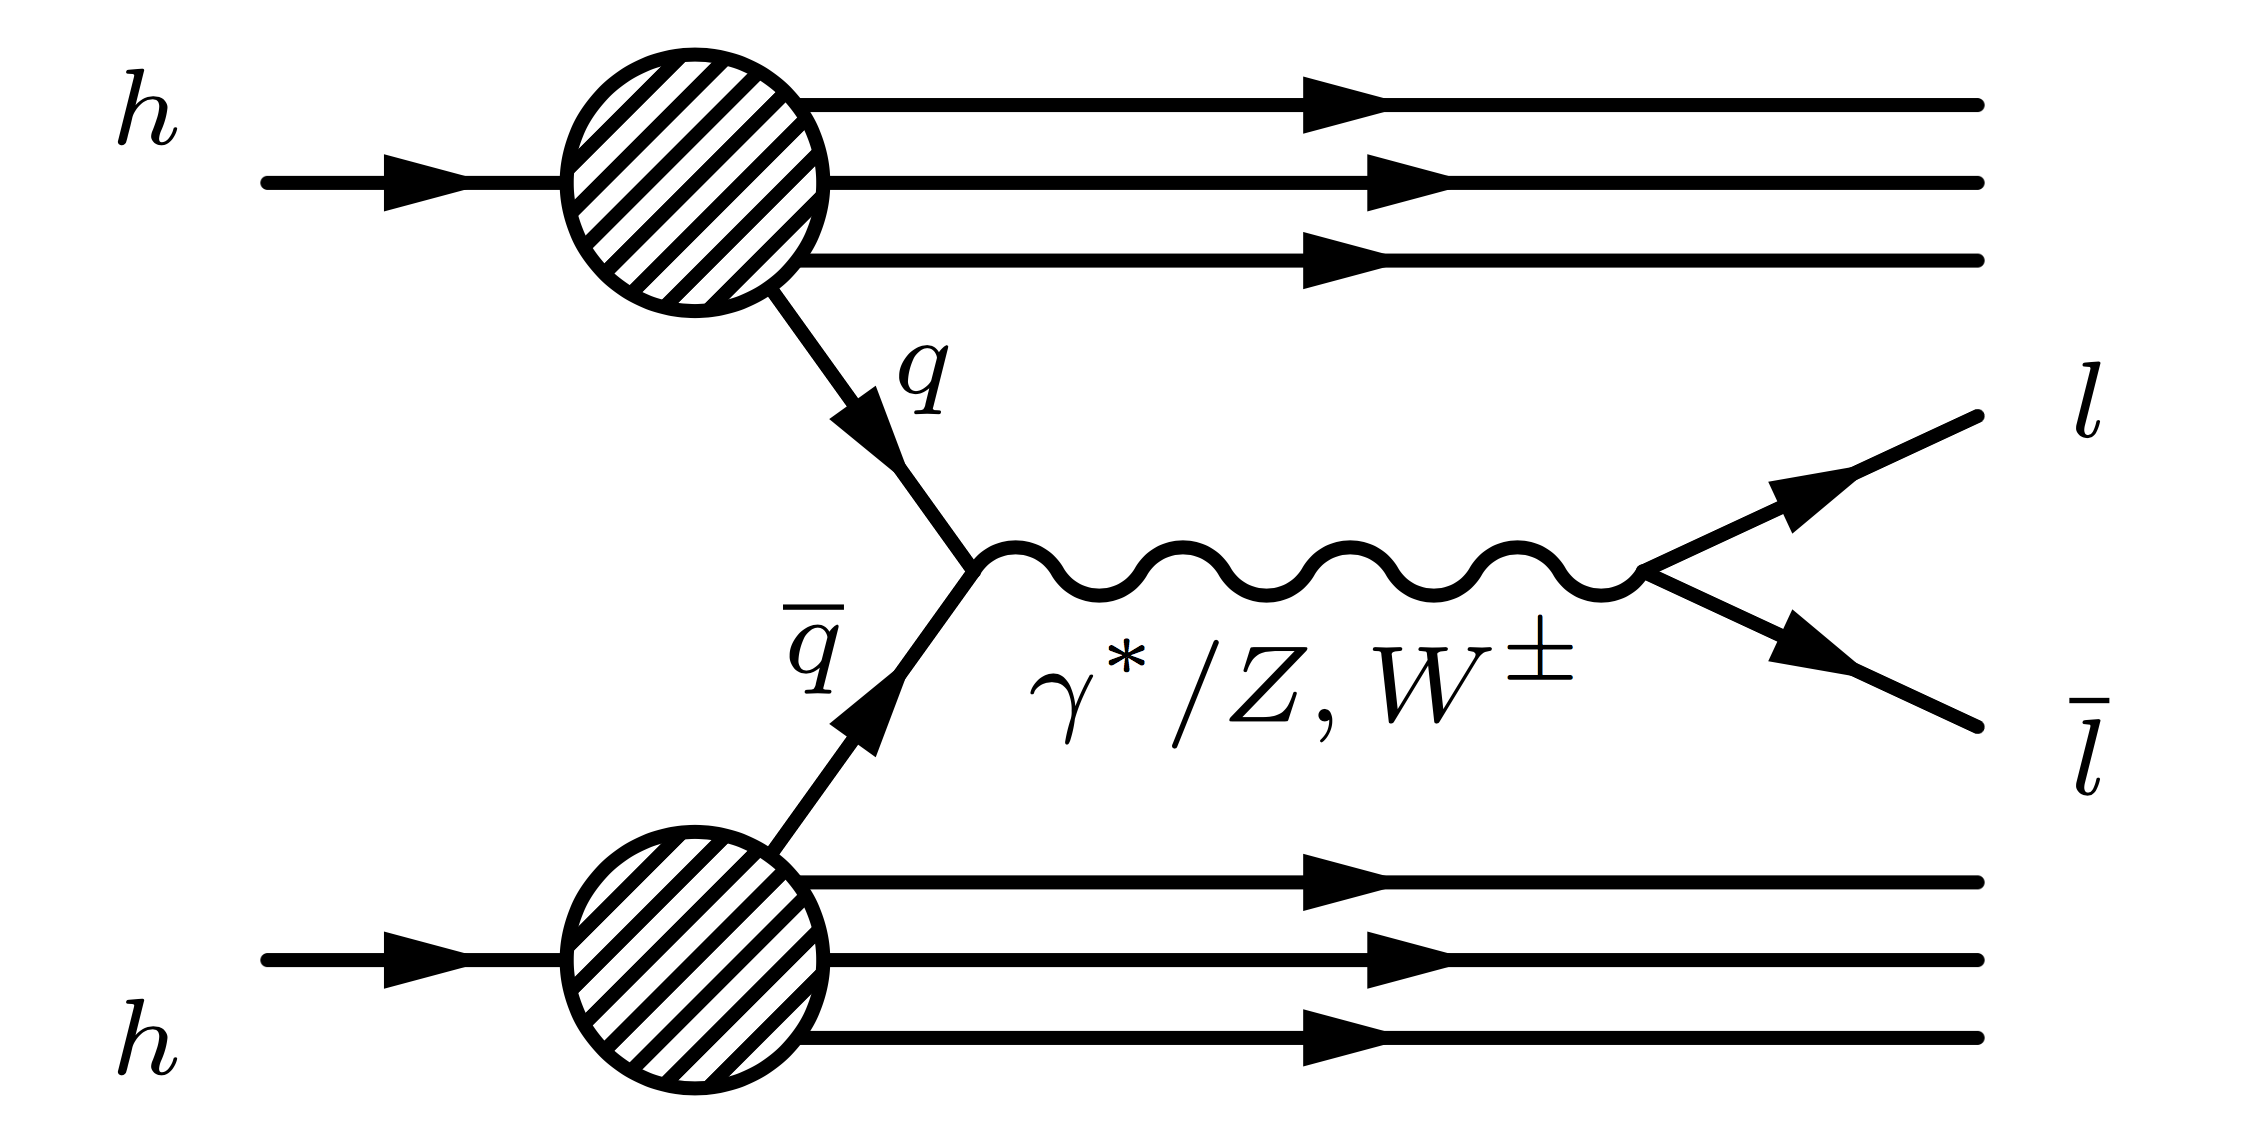
\includegraphics[width=0.7\linewidth]{Theory/DY.png} }
\caption{A schematic representation of the W/Z production via Drell-Yan process in a hadron collider.}
\label{fig:DY}
\end{figure}

In analogy to this process, the on-shell production of W and Z bosons using Drell-Yan reaction can be calculated as:
\begin{equation}
\hat{\sigma}^{q\bar{q}' \to W} = \frac{\pi}{3}\sqrt{2}G_F M^2_W | V_{q\bar{q}'}|^2 \delta (\hat{s}-M^2_{W}),
\end{equation}
\begin{equation}
\hat{\sigma}^{q\bar{q} \to Z} = \frac{\pi}{3}\sqrt{2}G_F M^2_Z (v^2_q+a^2_q) \delta (\hat{s}-M^2_{Z}),
\end{equation}
where the $q$ and $q'$ are the different quarks. The $V_{q\bar{q}'}$ is the appropriate Cabibbo-Kobayashi-Maskawa matrix element (describes a strength of flavor changing weak decays), and $v_q$ ($a_q$) the vector (axial vector) coupling of the Z-boson to the quarks. For the full production cross section, the partonic spectrum of colliding hadrons has to be considered. For two quarks, carrying fractions $x_1$ and $x_2$ of the colliding protons momenta, the momentum transfer $Q^2$ can be written as:
\begin{equation}\label{eq:Q2}
Q^2 = (x_1P_1 + x_2P_2) \approx x_1 x_2 \sqrt{s} = M^2_{Z,W,\gamma^{*}},
\end{equation}
where the parton masses have been neglected in the calculation,  the $\sqrt{s}$ in the Eq.~\ref{eq:Q2} is the center-of-mass energy of 2 hadrons:
\begin{equation}
s=(P_1+P_2)^2.
\end{equation}


Another Lorentz invariant variable, used to describe the parton parton scattering is the rapidity of the boson, defined as:
\begin{equation}
y = \frac{1}{2} log \frac{E+P_z}{E-P_z},
\end{equation}
where $E$ is the energy of the boson and $P_z$ is its $z$ component of the momentum.
This quantity can be connected to the momentum fraction carried by initial partons in a leading order approximation as:
\begin{equation}
x_{1,2}=\frac{M_{Z,W,\gamma^*}e^{\pm y}}{\sqrt{s}}.
\end{equation}
The maximum accessible rapidity range for the production of the bosons can be determined from the $\sqrt{s}$ and the mass of the boson as:
\begin{equation}
|y^{max}_{bos}| = ln \frac{\sqrt{s}}{M_{Z,W,\gamma^*}}.
\end{equation}

\begin{figure}[!tb]
\center{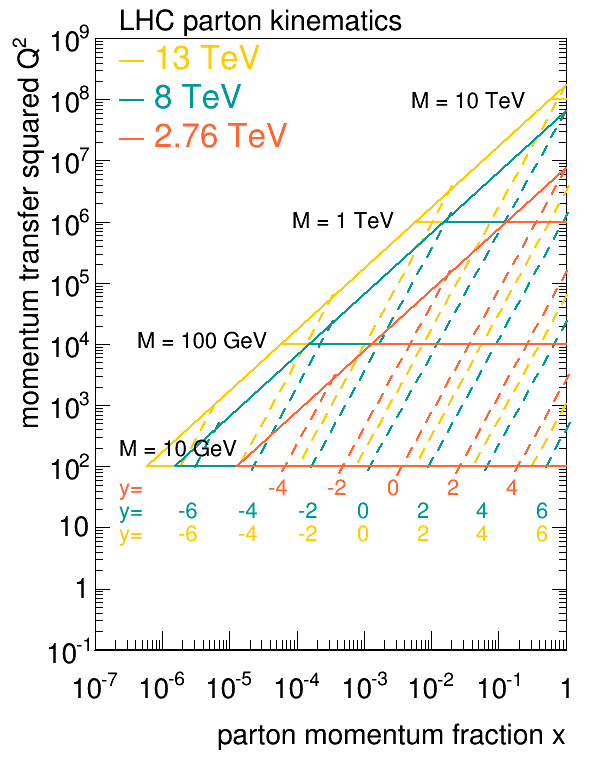
\includegraphics[width=0.7\linewidth]{Theory/LHCpartonkinematics.png} }
\caption{The parton kinematics accessible in the \atlas experiment in $Q^2$--$x$ plane. The limits are shown at $\sqrt{s}$ = 13 TeV, $\sqrt{s}$ = 8 TeV and $\sqrt{s}$ = 2.76 TeV\cite{partKin}.}
\label{fig:PartKin}
\end{figure}

The kinematic phase space of the proton, accessible at \atlas for different center-of-mass energies is shown in Fig.~\ref{fig:PartKin}. The W and Z cross sections at 2.76 TeV correspond to $Q^2\approx 10^4\,  GeV^2$ and therefore can probe the ranges of momentum fractions $x^{W}>8\cdot 10^{-4}$ and $x^{Z}>1 \cdot 10^{-3}$  for W and Z bosons respectively.  The $W^{+}$ production depends mainly on the $u$ and $\bar{d}$-quark distributions (the leading process is $u\bar{d}\to W^+$), the $W^{-}$ to $\bar{u}$ and $d$-quark distributions. The Z boson production cross section is most sensitive to the valence quark distributions.

The Drell--Yan process contributes to around 65\% of cross section \cite{Ellis:318585}, with both valence--sea and sea--sea quarks interactions included. The dominant higher order corrections are determined by the interaction of quarks with gluon (occurs in approximately 20\% of the events). 

Due to the very small lifetime of W and Z-bosons, this production is instantly followed by decay. 
The probability of a certain decay mode is described by the \textit{branching ratio}, $\textbf{BR}(X\to a+b)$, that is a fraction of a partial decay rate (of the decay mode of interest) and the total decay rate of the boson.  The W and Z-boson decay modes are summarized in Tab.~\ref{tab:WZDecayModes}. The W and Z bosons can decay hadronically with the production of a quark--antiquark pair for all quark flavors, except for top quark since its mass exceeds the mass of the bosons.  This mode of the decay is the dominant one because of the three possible color states for each quark. In a leptonic decay mode of the W-boson, the lepton plus corresponding same flavor neutrino/antineutrino  pair is produced. The leptonic decays of Z-boson create a lepton-antilepton pair. The visible fraction of Z-bosons decaying into leptons is smaller, compared to W, because of the invisible mode of Z-bosons decay, where a neutrino-antineutrino pair is produced. Because of the \textit{lepton universality} in the SM and large masses of W and Z-bosons ($M_Z > M_W \gg M_l$), the branching ratios of the leptonic decays are almost identical.

\begin{table}[!tbp]
\begin{center}
\caption{Branching ratios of the different W and Z decay modes \cite{Agashe:2014kda}. Invisible denotes the Z decays with a neutrino-antineutrino pair as a final state. The predicted values are estimated with sin$^2\theta_W = 0.23$.}
\label{tab:WZDecayModes}
\begin{tabular}{l | c | c | c }
\hline
Boson & Decay mode & Measured & SM \\
	& & branching ratio & prediction \\
\hline
$W$ & $e\nu_e$ & $(10.71\pm0.16)\%$ & \\
    & $\mu\nu_{\mu}$ & $(10.63\pm0.15)\%$ & 11.1\% \\
    & $\tau \nu_{\tau}$ & $(11.38\pm0.21)\%$ & \\
    & hadrons & $(67.41\pm0.27)\%$& 66.7\% \\
 \hline
 $Z$ & $e^+e^-$ & $(3.363\pm0.004)\%$ & \\
 	& $\mu^+\mu^-$ & $(3.366\pm0.007)\%$ & 3.4 \% \\
 	& $\tau^+ \tau^-$ & $(3.3658\pm0.008)\%$ & \\
 	& invisible & $(20.00\pm0.06)\%$ & 20.5\% \\
 	& hadrons & $(69.91\pm0.06)\%$ & 69.2\% \\
 \hline 
\end{tabular}
\end{center}
\end{table}

Due to experimental difficulty to measure the hadronic decays, the  W/Z cross sections are usually measured through their leptonic decay modes. The expected NNLO production cross sections times their branching ratios to one of the leptons is estimated using FEWZ program\cite{FEWZ} and CT14nnlo\cite{CT14}, at $\sqrt{s}$=2.76 TeV are:
\begin{equation}\label{eq:WcsNNLO}
\sigma^{NNLO}_{W^+ \to l \nu} = 2114^{+8}_{-11}(scale)\, ^{+57}_{-59}(PDF)\, [pb],
\end{equation}
\begin{equation}
\sigma^{NNLO}_{W^- \to l \nu} = 1265^{+5}_{-6}(scale)\, ^{+32}_{-38}(PDF)\, [pb]
\end{equation}
and 
\begin{equation}\label{eq:ZcsNNLO}
\sigma^{NNLO}_{Z^- \to ll} = 304^{+1}_{-1}(scale)\, ^{+7}_{-7}(PDF)\, [pb],
\end{equation}
where the the first uncertainty comes from the uncertainty of the scale choice. The second uncertainty arises from the imperfect knowledge of proton PDFs. The difference between $W^{+}$ and $W^{-}$ cross sections (called charge asymmetry) is due to  the higher probability of finding a $u$--quark rather than $d$--quark in the proton.

The NNLO QCD predictions of W and Z-boson cross sections in $pp$ and $p\bar{p}$ collisions together with the results obtained using different experiments are shown in Fig.~\ref{fig:Zcs}. It can be observed, that the W and Z-boson cross sections have not been measured so far in the region around 1 TeV < $\sqrt{s}$ < 7 TeV in pp collisions.


\begin{figure}[!tbp]
\begin{minipage}[h]{1.0\linewidth}
\center{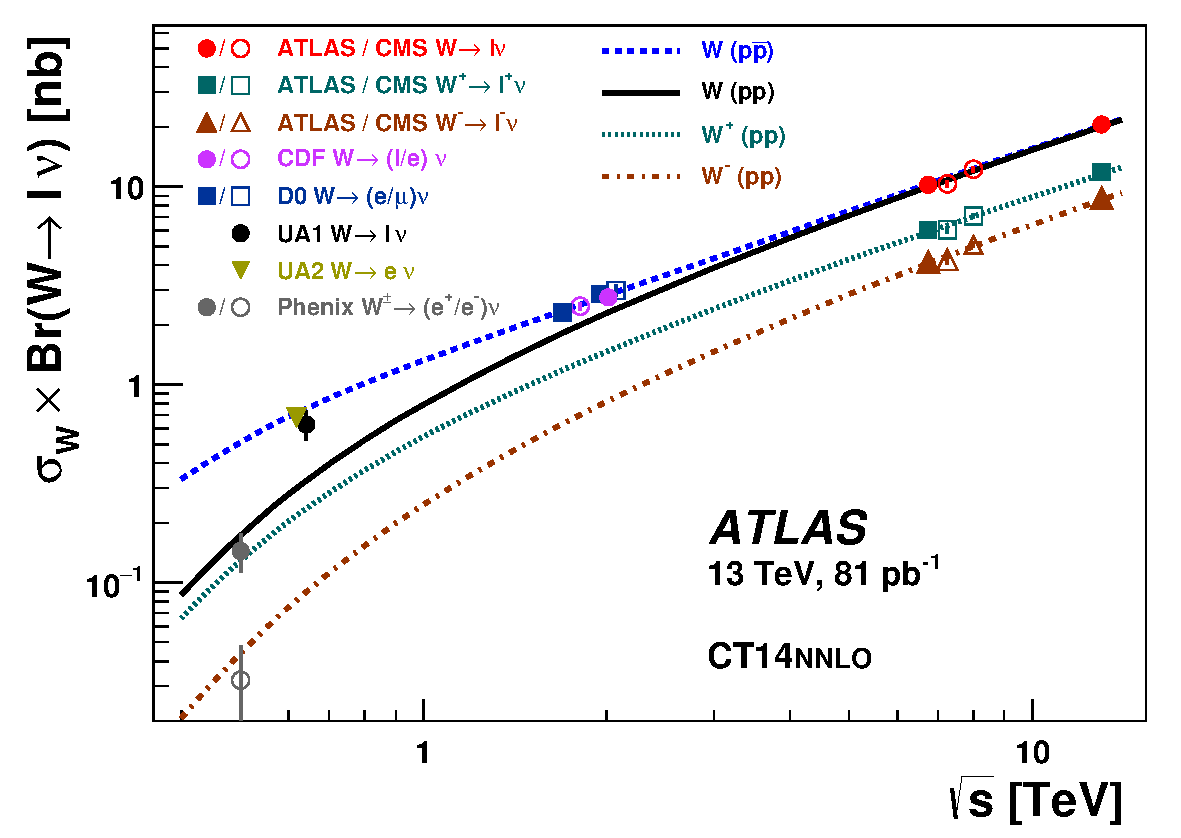
\includegraphics[width=0.7\linewidth]{Theory/Wcs.pdf} \\ a)}
\end{minipage}
\vfill
\begin{minipage}[h]{1.0\linewidth}
\center{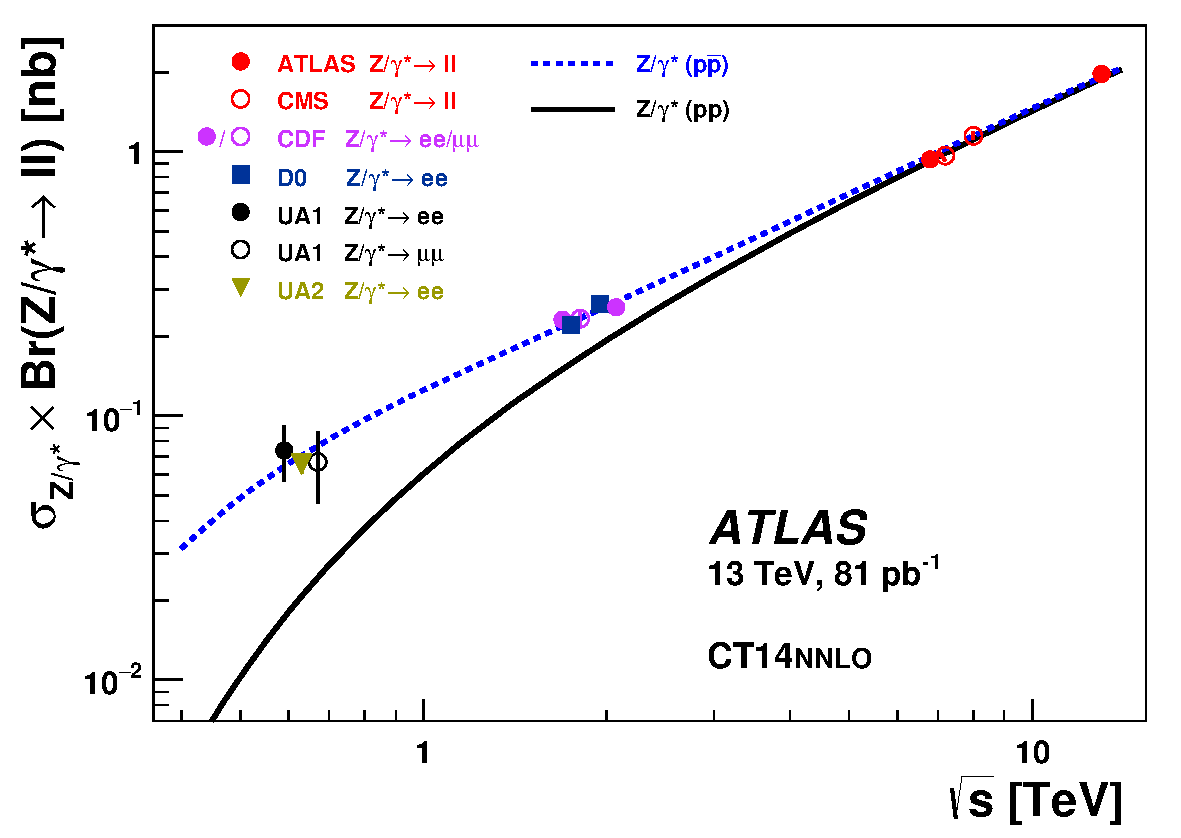
\includegraphics[width=0.7\linewidth]{Theory/Zcs.pdf} \\ b)}
\end{minipage}
\caption{The measured values of a) $\sigma_{W \to l\nu}$ and b) $\sigma_{Z \to ll}$ compared to the theoretical predictions based on NNLO QCD calculations. The predictions and previous measurements are shown for both proton-proton and proton-antiproton colliders as a function of $\sqrt{s}$.  All data points are displayed with their total uncertainty. The calculations were performed with the program FEWZ using the CT14nnlo parton density function parameterization. The theoretical uncertainties on the cross section predictions are not shown. Figure taken from \cite{a13TeV}.}
\label{fig:Zcs}
\end{figure}

